\documentclass{article}
\usepackage{float}
\usepackage{amsmath}
\usepackage{longtable}
\usepackage[margin=1in]{geometry}
\usepackage{caption}
\usepackage{booktabs}
\usepackage[dvipsnames]{xcolor}
\usepackage{fancyvrb}
\usepackage{graphicx}
\usepackage{indentfirst}
\RecustomVerbatimCommand{\VerbatimInput}{VerbatimInput}%
{fontsize=\footnotesize,
 %
 frame=lines,  % top and bottom rule only
 framesep=2em, % separation between frame and text
 rulecolor=\color{Gray},
 %
 label=\fbox{\color{Black}Profiling Result},
 labelposition=topline,
 %
 commandchars=\|\(\), % escape character and argument delimiters for
                      % commands within the verbatim
 commentchar=*        % comment character
}

\begin{document}
\title{STA663 Final Project \\ Indian Buffet Process and its application in the Infinite Latent Feature Model}
\author{Dipesh Gautam}
\date{\today}
\maketitle

\section{Background}
\subsection{Indian Buffet Process (IBP)}
The Indian Buffet is an adaptation of Chinese Buffett Process where each object instead of being associated with a single latent class can  be associated with multiple classes. This is particularly useful when each object has multile latent features and by associating objects with a single class we cannot partition them into homogeneous subsets.

In the Indian buffet process, $N$ customers enter a restaurant one after another. Each customer encounters a buffet 
consisting of infinitely many dishes arranged in a line. The first customer starts at the left of the buffet and 
takes a serving from each dish, stopping after a Poisson($\alpha$) number of dishes. The $i$th customer moves along the buffet, 
sampling dishes in proportion to their popularity, taking dish $k$ with probability $\frac{m_k}{i}$ , where $m_k$ is the number of 
previous customers who have sampled that dish. Having reached the end of all previous sampled dishes, the $i$th customer 
then tries a Poisson($\frac{\alpha}{i}$) number of new dishes. Which costumer chose which dishes is indicated using a binary matrix \textbf{Z} with $N$ rows and infinitely many columns(corresponding to the infinitely many selection of dished), where $z_{ik}$ = 1 if the $i$th costumer sampled $k$th dish.


\section{Implementation}
IBP can be used as a prior in models for unsupervised learning. An example of which is presentd in Griffiths and Ghahramani(2005) and Yildirim(2012), where IBP is used as a prior in infinite linear-gaussian model.

\subsection{Infinite Latent Features Model}
We used the linear-gaussian feature model as derived in Griffiths and Ghahramani(2005). We consider a binary feature ownership matrix $Z$ which represents the presence or absence of the underlying features of the observations $X$. Thus each D-dimensional object $x_i$ is generated from a Gaussian distribution:
\[
x_i \sim Normal(z_iA, \Sigma_X)
\]
Where A is $KXD$ matrix of weight representing the $K$ latent features and $\Sigma_X= \sigma^2_xI$ is the covariance matrix that introduces white noise to the images. The weight matrix $A$ itself has a prior with mean 0, and covariance $\sigma^2_AI$. Thus, the likelihood is given for the data is given by:
\begin{multline}\label{eq:lik}
P(X|Z,\sigma_X, \sigma_A) = \frac{1}{(2 \pi)^{ND/2} (\sigma_X)^{(N-K)D}(\sigma_A)^{KD}(|Z^TZ+\frac{\sigma_X^2}{\sigma_A^2}I|)^{D/2}}\\
exp\{-\frac{1}{2\sigma_X^2}tr(X^T(I-Z(Z^TZ+\frac{\sigma_X^2}{\sigma_A^2}I)^{-1}Z^T)X)\}
\end{multline}


\subsection{Algorithm for Gibbs sampling and Metropolis-Hastings}

\subsubsection{Parameters}
The parameters of interest are:
\begin{itemize}
\item{Z: feature ownership matrix}
\item{$K_{new}$: Number of new features}
\item{$\alpha$: parameter $K_{new}$}
\item{$\sigma_X$}
\item{$\sigma_A$}
\end{itemize}

Full conditionals can be obtained for $Z$, $K_{new}$ and $alpha$, so, we can update them using Gibbs sampling. For $\sigma_X$ and $\sigma_A$, we'll use random walk MH algorithm for updating.\\
\subsubsection{Priors for $Z$, $K_{new}$ and $\alpha$}

Gamma prior is set for $\alpha$
\begin{equation}\label{eq:prioralpha}
\alpha \sim Gamma(1,1)
\end{equation}

Prior on \textbf{Z} is obtained by IBP as:
\begin{equation}\label{eq:priorZ}
P(z_{ik}=1|\textbf{z}_{-i,k}) = \frac{n_{-i,k}}{N}
\end{equation}

$K_{new}$ has a poisson prior:
\begin{equation}\label{eq:priork}
K_{new} \sim Poisson(\frac{\alpha}{N})
\end{equation}



\subsubsection{Full conditional posteriors on $Z$, $K_{new}$ and $\alpha$}
Full conditional posterior for Z can be directly computed using Equations \eqref{eq:lik} and \eqref{eq:priorZ} as given below:
\begin{equation}\label{eq:postZ}
P(z_{ik}|X,Z_{-(i,k),},\sigma_X,\sigma_A) \propto  P(X|Z,\sigma_X, \sigma_A) * P(z_{ik}=1|\textbf{z}_{-i,k}) 
\end{equation}

Full conditional posterior for $\alpha$ is given by:
\begin{equation}\label{eq:postalpha}
P(\alpha|Z) \sim Gamma(1+K_+,1+\sum_{i=1}^{N} H_i)
\end{equation}

To sample the number of new features for observation $i$, we use a truncated distribution, computing probabilities for a range of values $K_{new}^{(i)}$ up to an upper bound (say 3). Using the ikelihood and prior given by Equations \eqref{eq:lik} and \eqref{eq:priork} respectively, we can easily calculate the probability distribution for $K_{new}$ and sample the number of new dishes accordingly.
%\begin{equation}\label{eq:postk}
%P($K_1$|X, Z, $\sigma_X$, $\sigma_A$) \sim P($K_{new}$)*P(X|Z,\sigma_X, \sigma_A)
%\end{equation}




\subsubsection{Metropolis-Hastings for $\sigma_X$ and $\sigma_A$}
For $\sigma_X$ we use random-walk MH algorithm as follows:
\begin{eqnarray}
\epsilon \sim Uniform(-.05,.05)\\
\sigma_X^{*} =  \sigma_X +\epsilon\\
\end{eqnarray}

Accept this new $\sigma_X$ with probability given by:
\begin{equation}
AR = min\{1,\frac{P(X|Z, \sigma_X^{*}, \sigma_A)}{P(X|Z, \sigma_X,\sigma_A)}\}\\
\end{equation}

Where AR is the acceptance ratio.

We use similar algorithm to sample $\sigma_A$ where we replace $\sigma_X$ by $\sigma_A$ in the algorithm described above.



\section{Unit Testing}

\section{Profiling and Optimization}
We profiled the code using \textit{cProfile} to figure out bottlenecks. The result is shown in \textit{Profiling result}. We see that most of the computational time is spent on calculating the \textit{log likelihood(ll)}  and matrix inversion. Due to this fact, one of the first things we looked at were ways to reduce computation time for likelihood and/or inverse calculation.\\

\VerbatimInput{profiler.txt}

\subsection{Matrix Inversion}
We tried the matrix inversion method described in Griffiths and Ghahramani(2005, eq 51-54), where the method reduces the runtime by allowing us to perform rank one updates instead when only one value is changed. We implemented the algorithm and were able to speed up the process as shown in Table \ref{compareInverse}.

\begin{table}[ht]
\centering
\caption{Comparision of matrix inverse methods \label{compareInverse}}
\begin{tabular}{lr}
\toprule
{} &      Time \\
\midrule
linalg.inverse &  0.000078 \\
calcInverse    &  0.000036 \\
\bottomrule
\end{tabular}

\end{table}

Even though we were able to improve the performance, due to some numerical errors, we were not able to obtain a stationary MCMC chain using this method. This could be achieved by spending some more time on it but due to time constraints we decided that to look at fixing this at a later time.\\

\subsection{Likelihood function}
While working on the optimized matrix inversion, we noticed that the matrix that we're inverting i.e. ($Z^TZ+\frac{\sigma_X^2}{\sigma_A^2}I$) actually appears twice inside the likelihood function. So, we looked at removing the redundancy by calculating the matrix and storing it. We were able to gain some improvement using this method as shown in Table \ref{llcomp} and Table \ref{runtimes}. Since the likelihood function is called numerous times, even the small gain shwon in Table \ref{llcomp} was translated into a substantial gain as shown in Table \ref{runtimes}.\\


\begin{table}[ht]
\centering
\caption{Runtime Comparision \label{llcomp}}
\begin{tabular}{lr}
\toprule
{} &      Time \\
\midrule
original ll function &  0.000392 \\
Proposed ll function &  0.000337 \\
\bottomrule
\end{tabular}


\end{table}

\subsection{Cython}
Another way we looked at improving the performance of the code was by cythonizing the code. We again looked at improving the performance of the likelihood function by cythonizing it. As shwon in Table \ref{runtimes}, we were not able to gain substantial improvements from it.\\


\subsection{Parallelization and CUDA}
Since our algorithm is an MCMC algorithm with serial dependence, parallelization does not seem to be a good idea. One of the ways, parallelization can be done is by splitting the chain into multiple smaller chains and combining them back. We tested it and it showed some improvement in the code but decided against using it as the gain wasn't significant enough as we had to take care of multiple burn-in periods and ignore the loss of markov property due to multiple chains. Also, parallelizing the density calculation for likelihood wasn't an option for our algorithm as we had a discrete density with just two points.


\begin{table}[ht]
\centering
\caption{Runtime Comparision \label{runtimes}}
\begin{tabular}{lr}
\toprule
{} &  Total Time \\
\midrule
Initial Code &  539.818143 \\
Improved ll  &  489.207815 \\
Cythonized   &  507.522965 \\
\bottomrule
\end{tabular}

\end{table}


\section{Application and Results}
\subsection{Simulated Data}
We used simulated data similar to Griffiths and Ghahramani(2005) and Yildirim (2012). The data set consists of 100($N$) images $X$, where each image $x_i$ a vector of length 36($D$) representing the $6X6$ dimension of each object. These images were created using 4($K$) latent features (base images) which correspond to the rows of the weight matrix $A$. Each object has .5 probability for presence of each feature. Then the object was created by adding white noise corresponding to $\sigma_X^2=0.5$ as:
\[
x_i \sim Normal(z_iA, \sigma_X^2I)
\]
The basis image and first four simulated images are shown in Fig. \ref{fig:original}, where the top row are the features, bottom row are the first four objects and the middle row represents presence or absence of each of the four features.\\

\subsection{Results}
\subsubsection{Validation and $K_+$}
We ran our sampler with the improved likelihood calculation for 1000 iterations. Our data was simulated with 4 latent features. The distribution of $K_+$(total features detected at each iteration) is shown in Fig. \ref{fig:dist}(a). Although we see that the mode of the number of features is 5, with significant iterations where the number of features is 7, we can see from Fig. \ref{fig:dist}(b) that most of the objects actually had between 1 and 4 features with very few of them with 5 or more features. These outliers can be attributed to the noise and variance in the data simulation and ignored. So, we can conclude that the algorithm correctly predicts and detects the existence of 4 latent features in the simulated data.\\
Trace plot for $\sigma_X$, $\sigma_A$, and $\alpha$ is shown in Fig. \ref{fig:trace}. We see that $\sigma_X$ is converging to it's true value of $0.5$ and the other parameters also show proper convergence validating the authenticity of the algorithm.\\ 
\begin{figure}[ht]
\caption {Distribution of Kplus and mean number of features per object}
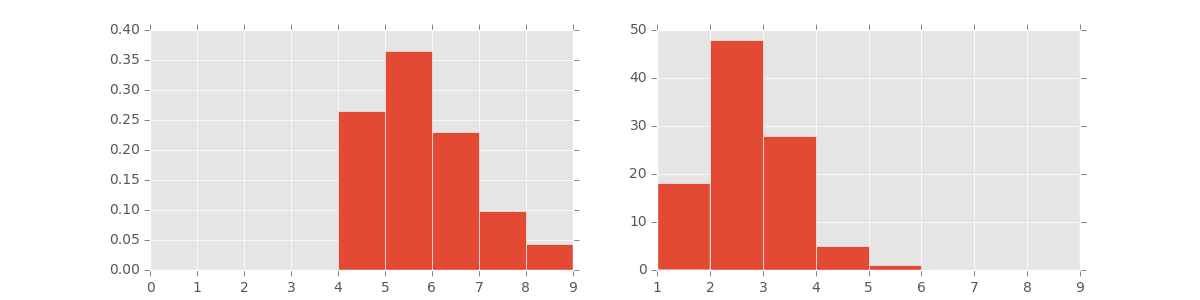
\includegraphics[width=\linewidth]{figures/kDistribution.png}
\label{fig:dist}
\end{figure}

\begin{figure}[ht]
\caption {Traceplots for $\sigma_X$, $\sigma_A$ and $\alpha$}
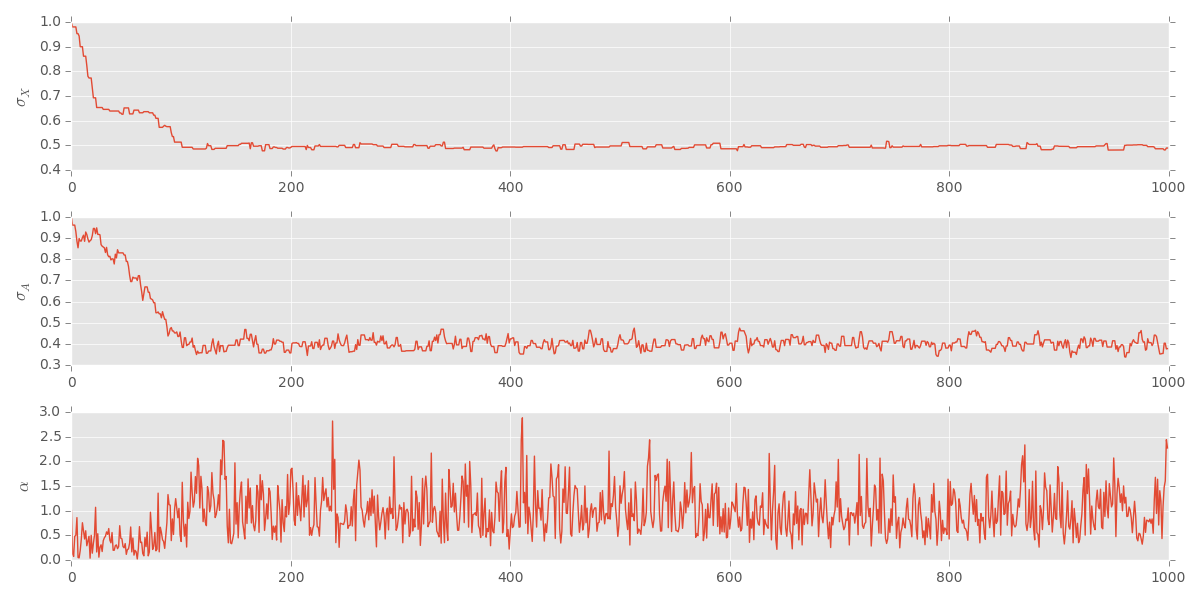
\includegraphics[width=\linewidth]{figures/Trace.png}
\label{fig:trace}
\end{figure}

\subsubsection{Latent features and recreating objects}
Posterior estimation of $A$ is given by:
\[
E[A|X,Z] = (Z^TZ+\frac{\sigma_X^2}{\sigma_A^2}I)^{-1}Z^TX
\]
as givin in Griffiths and Ghahramani(2005) eq.59. For this calculation, we used the final Z obtained from the MC using only the first four columns corresponding to the four detected features. Likewise, posterior mean of $\sigma_X$ and $\sigma_A$ was used in the calculation of posterior expectation of weight matrix A.\\
With this information and the posterior Z, we were able to recreate the objects X as:
\[
Xi \sim Normal(ZiA,0)
\]
We used zero variance to ignore the white noise in the recreated images. The results are shown in Fig. \ref{fig:detected}. By comparing with the original features and simulated objects as given in Fig. \ref{fig:original} with the detected features and recreated objects as given in Fig. \ref{fig:detected}, we can conclude that the algorithm was successfull in identifying all the latent features and successfully detecting the presense or absence of those features in the simulated objects which had white noise making detection difficult.


\begin{figure}
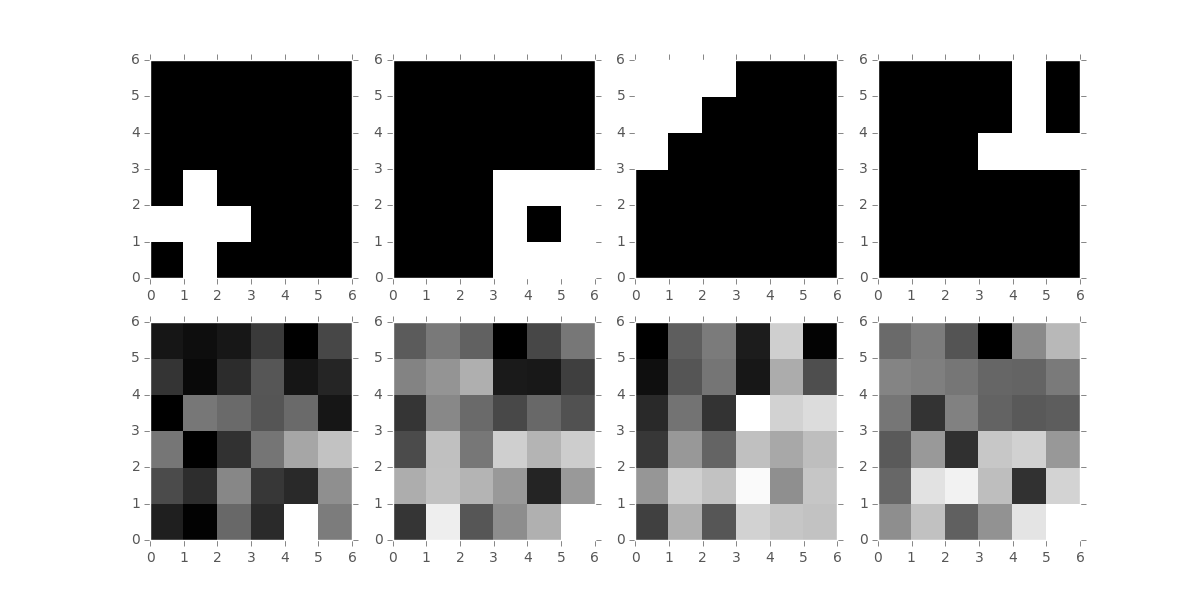
\includegraphics[width=\linewidth]{figures/Original.png}
\caption {Original Features, First four simulated objects and the features present in each of the objects. First row shows the 4 latent features used to simulate the data. Third row shows the first four simulated objects and the middle row shows the presense or absence of the the latent features (in the order specified in the first row) in the corresponding objects below. Light signifies presence and dark signifies the absence of the feature for any given object.}
\label{fig:original}
\end{figure}



\begin{figure}
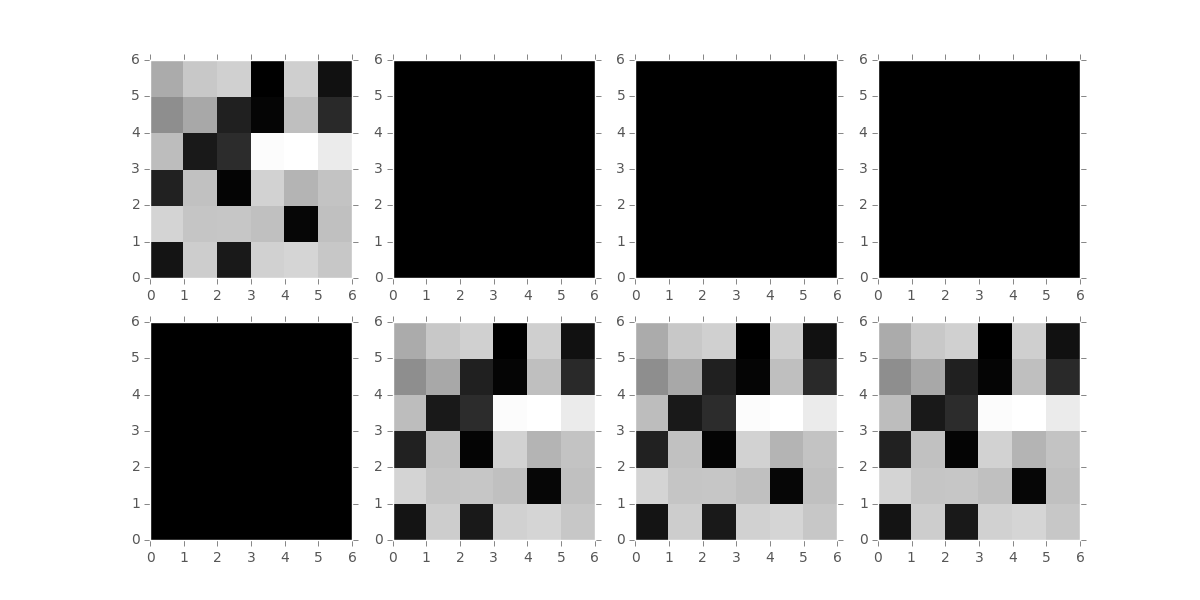
\includegraphics[width=\linewidth]{figures/Detected.png}
\caption {Detected Features, First four recreated objects and the features present in each of the objects. First row shows the 4 latent features used detected by MCMC. Third row shows the first four recreated objects and the middle row shows the presense or absence of the the latent features (in the order specified in the first row) in the corresponding objects below. Light signifies presence and dark signifies the absence of the feature for any given object.}
\label{fig:detected}
\end{figure}

\section{Comparision}

\section{Conclusions}



\end{document}
